% !TEX root = ../thesis-example.tex
%
\chapter{Theorie/Begriffsbestimmung}
\label{sec:theorie:Theorie}

\cleanchapterquote{Most good programmers do programming not because they expect to get paid or get adulation by the public, but because it is fun to program.}{Linus Torvalds}{(Finnish American, software engineer and hacker)}

Zur Gewährleistung des allgemeinen Verständnisses, werden einige grundlegende Begriffe definiert, welche die Grundlage für die folgende Untersuchung bilden.

Die Entscheidung, welche mobile Variante für die Umsetzung verwendet werden soll, ist abhängig von den jeweiligen Eigenschaften der Anwendungen:

\begin{itemize}
	\item Wieviel Speicher steht der App zur Verfügung?
	\item Welche Handyfunktionen werden benötigt?
	\item Lässt sich feststellen wann eine Internetverbindung besteht?
	\item Lassen sich die Daten, abhängig von einer bestehenden Internetverbindung, mit dem Server abgleichen.
\end{itemize}

Die nachfolgenden Vor- und Nachteile von Nativen Apps, Web Apps und Hybrid Apps sind auf der Website www.app-entwickler-verzeichnis.de beschrieben.\cite[]{WEB:APPEV:2014}

\section{Native Apps}
\label{sec:intro:native}

Die Nativen Apps werden speziell für das jeweilige Betriebssystem entwickelt z.B. iOS oder Android. Diese laufen dann auch ausschließlich auf iOS Geräten wie dem iPhone und dem iPad, oder Android Geräten wie dem Samsung Galaxy S4.

Dadurch wird eine optimale Nutzung der Ressourcen und einheitlich funktionierende Hardwareschnittstellen sichergestellt.

\subsection{Vorteile}
\label{sec:native:pros}

\begin{itemize}

	\item Native Apps nutzen die Leistung des Betriebssystems und des verwendeten Gerätes voll aus, da sie speziell für das Betriebssystem angepasst sind. Dadurch lassen sich sehr gut komplexere und rechenintensivere Apps umsetzen.

	\item Durch die Installation der Apps auf dem Endgerät können Hardwarefunktionen wie Kamera, Beschleunigungssensor oder \ac{GPS} benutzt werden. Das ist in der Regel nur nativen Apps vorbehalten.

	\item Daten können auf dem Endgerät in beliebiger Menge gespeichert werden.

	\item Da Native Apps über einen Appstore vertrieben werden, wirken sich positive Bewertungen stark auf den Verkauf aus.

	\item Die App lässt sich sehr einfach über den Appstore installieren. Nach der Installation wird automatisch ein Icon zum Starten auf dem Homescreen angelegt.

	\item Der Vertriebsaufwand ist sehr gering, da die Appstores verbreitete Bezugsquellen für Native Apps sind. Ist die App erfolgreich, findet sich diese in den Top-Listen der App Stores wieder und erreicht dadurch sehr hohe Downloadzahlen.

\end{itemize}

\subsection{Nachteile}
\label{sec:native:cons}

\begin{itemize}

	\item Ein großer Nachteil ist der erforderliche Entwicklungsaufwand, wenn die App in allen Appstores angeboten werden soll, da die App an die jeweiligen Gegebenheiten des Betriebssystems optimiert werden muss.

	\item Es entstehen zusätzliche Kosten, um die App für den entsprechenden Appstore entwicklen und anbieten zu können.

\end{itemize}

\section{Web Apps}
\label{sec:intro:webapp}

Web Apps sind im eigentlichen Sinne speziell programmierte \ac{HTML5} Websites, die automatisch erkennen auf welchem Endgerät sie aufgerufen werden und optimieren den Inhalt entsprechend automatisch. Somit kann jedes mobile Endgerät, welches über einen Webbrowser verfügt, die App nutzen.

\subsection{Vorteile}
\label{sec:webapp:pros}

\begin{itemize}

	\item Web Apps sind quasi unabhängig vom Betriebssystem und funktionieren auf allen Smartphones. Dadurch werden mehr potentielle Nutzer bei gleichzeitig geringeren Kosten erreicht.

	\item In der Regel ist die Entwicklung einer Web App günstiger, als die Entwicklung einer nativen App für nur ein Betriebssystem.

	\item Durch die Verwendung von HTML5 wird auch die Offline-Speicherung von Daten ermöglicht. Somit kann nach erstmaligem laden die App auch ohne permanente Internetverbindung genutzt werden.

	\item Über Onlinesuchmaschinen wie beispielsweise Google können Web Apps ohne großen Aufwand gefunden und ohne Installation direkt genutzt werden. Werden diese als Lesezeichen gespeichert, lässt die Web App sich genau wie eine Native App vom Startbildschirm aus starten.

	\item Die Veröffentlichung und Aktualisierung einer Web App erfolgt in Sekundenschnelle, da sie im Gegensatz zu Nativen Apps keinen Zulassungsprozess durchlaufen muss.

	\item Vertreibt man die App selbst, entfällt die Provision von überlicherweise 30 Prozent an den Betreiber des App Stores.

\end{itemize}

\subsection{Nachteile}
\label{sec:webapp:cons}

\begin{itemize}

	\item Viele Hardwarefunktionen wie beispielsweise die Kamera oder das \ac{GPS} der mobilen Geräte lassen sich garnicht oder nur mit spezieller Zustimmung des Nutzers verwenden.

	\item Komplexe Berechnungen wie beispielsweise 3D Darstellungen, Verschlüsselungen oder Bildbearbeitungen sind mit einer Web App nicht möglich.

	\item Benötigt die App mehr als 10MB an Datenmaterial auf dem Endgerät, ist von einer Entwicklung als reine Web App abzusehen.

	\item Geschäftsmodelle, die auf In-App-Käufe oder einem App Store aufbauen, funktionieren zusammen mit der Web App nicht.

\end{itemize}

\section{Hybridapps}
\label{sec:intro:hybrid}

Hybridapps haben das Ziel, die Vorteile der Web App Entwicklung und der Entwicklung nativer Apps in sich zu vereinen. Dabei setzen die Entwickler auf eine große Anzahl von Frameworks. PhoneGap, Corona oder Appelerator Titanium sind Beispiele für Frameworks, mit deren Hilfe Web Apps in eine native App umgewandelt werden kann.

Hybrid Apps besitzen jedoch auch Vor- und Nachteile.

\subsection{Vorteile}
\label{sec:hybrid:pros}

\begin{itemize}

	\item Durch die Verwendung einer Hybrid App lässt sich eine Cross Browser Web App erstellen, die in allen modernen Browsern läuft.

	\item Da eine Web App mittels Frameworks für verschiedene Betriebssysteme umgewandelt werden kann, bleibt die eigenständige Entwicklung für jedes einzelne Betriebssystem erspart. Es bleiben im schlimmsten Fall nur betriebssystemspezifische Feinheiten, die noch angepasst werden müssen.

	\item Mit Javascript lassen sich viele Hardwarefunktionen der mobilen Endgeräte nutzen, auf die man bei einer Web App nicht zugreifen konnte.

	\item Der Verkauf einer Hybrid App erfolgt über den jeweiligen App Store.

\end{itemize}

\subsection{Nachteile}
\label{sec:hybrid:cons}

\begin{itemize}

	\item Ein großer Nachteil einer Hybrid App kann entsteht, wenn sehr rechenintensive Anwendungen verwendet werden. Dadurch erreichen Hybrid Apps sehr schnell ihr Leistungsmaximum reagieren träge. Dies ist sehr stark vom verwendeten Framework abhängig. Dieser Nachteil kann in Zukunft durch merklich effizienter werdende Frameworks behoben werden.

	\item Die Progammierung einer Hybrid App kann mit zunehmendem Komplexitätsgrad sehr aufwendig werden und dadurch eine Umsetzung mittels nativer App empfehlenswerter machen.

\end{itemize}

\section{Wahl der Appvariante}
\label{sec:intro:Appvariante}

Die Wahl der Appvariante ist nicht allein abhängig von den Vor- und Nachteilen der einzelnen Varianten. Hierfür muss auch die bestehende Website ``http://www.thueringen-tourismus.de/barrierefrei'' betrachtet und die Umsetzungsaufwände gegeneinander abgewägt werden.

Ein nicht zu unterschätzender Vorteil der Website ist die bereits responsive Umsetzung. (Abb.\ref{Barrierefreidatenbank}-\ref{Websitemobil}) Mit dieser passt sich der dargestellte Inhalt an die Auflösung des Endgeräts an, wodurch die optimale Darstellung auch auf mobilen Geräten gewährleistet wird. Es können somit bereits neue Daten für die Barrierefreiheitsdatenbank mobil erfasst werden.

\begin{figure}[htb]
	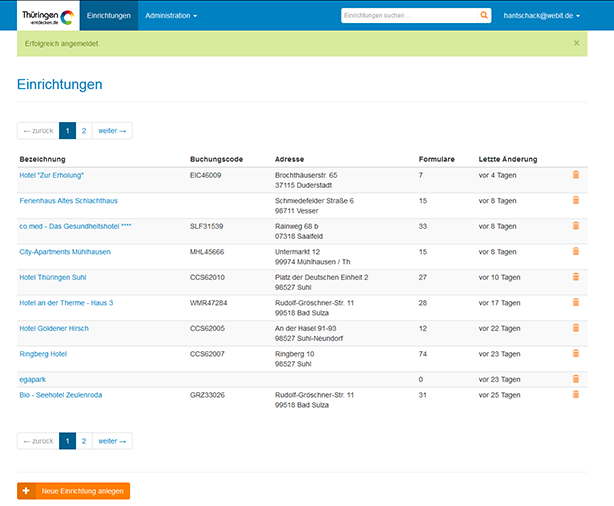
\includegraphics[width=\textwidth]{Bilder/Barrierefreidatenbank}
	\caption{Die Abbildung zeigt den Aufbau der Website http://www.thueringen-tourismus.de/barrierefrei auf der Daten für die Barrierefreiheitsdatenbanke eingepflegt und abgerufen werden können.}
	\label{Barrierefreidatenbank}
\end{figure}

\begin{figure}[htb]
	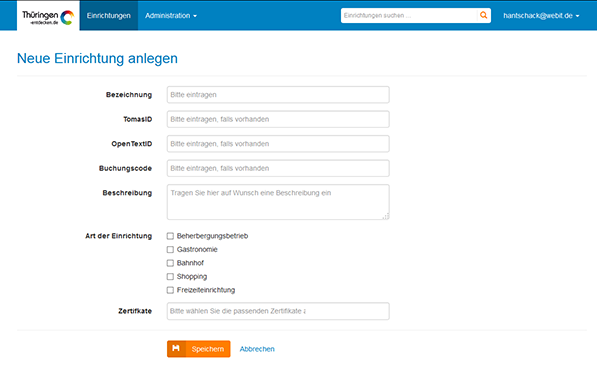
\includegraphics[width=\textwidth]{Bilder/Datenerfassung}
	\caption{In der Abbildung ist ein Standardformular zu sehen, welches grundlegende Eigenschaften für die Datenerfassung einer Einrichtung erhält. Wie beispielsweise die Art der Einrichtung.}
	\label{Datenerfassung}
\end{figure}

\begin{figure}[htb]
	\begin{tabular}{l r}
		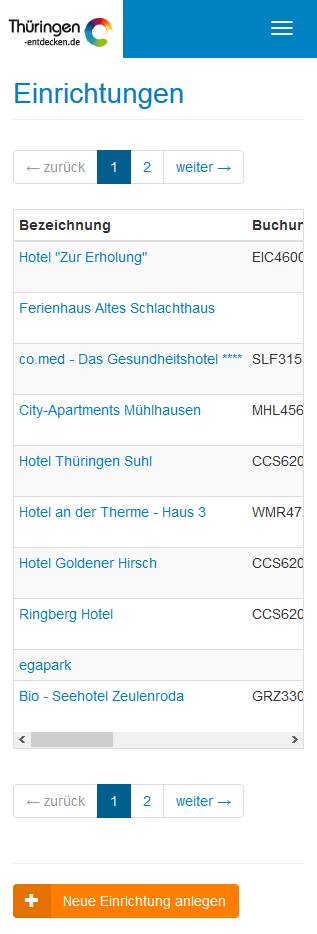
\includegraphics[width=0.49\textwidth]{Bilder/Barrierefreidatenbank-mobil}
		&
		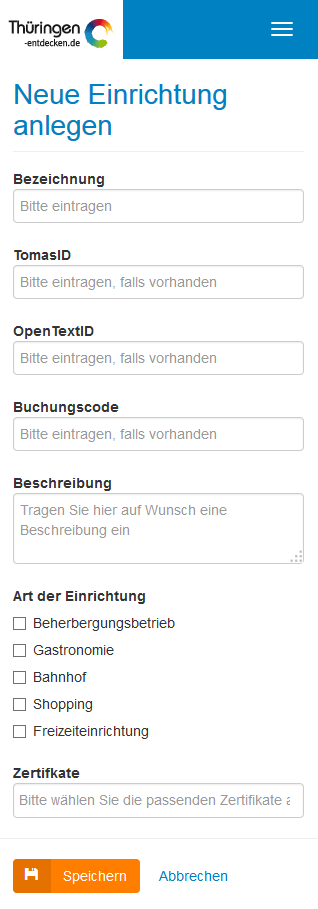
\includegraphics[width=0.49\textwidth]{Bilder/Datenerfassung-mobil}
	\end{tabular}
	\caption{Auf den beiden oberen Bilder ist sowohl die Ausgabe der erfassten Daten, als auch die Seite zur Datenerfassung auf einem mobilen Endgerät zu sehen. Navigation und Inhaltselemente passen sich an die Auflösung des Endgeräts an.}
	\label{Websitemobil}
\end{figure}

\cleardoublepage

Nach Betrachtung der Vor- und Nachteile der drei App Varianten und der bestehenden Website, bietet sich die Umsetzung einer reinen nativen App für die Datenerfassung der Barrierefreiheitsdatenbank nicht an. Der Umsetzungsaufwand und die entstehenden Kosten wären unangemessen hoch im Vergleich zu den daraus entstehenden Vorteilen.

Die responsive Variante der Website bietet sich auch nicht an, da sie eine permanente Internetverbindung voraussetzt.

Da eine Web App auf \ac{HTML5} aufbaut und die Website sich bereits teilweise an das Endgerät anpasst, baut die Untersuchung im zweiten Teil der Arbeit auf eine Umsetzung als Web App auf. Daher wird bei der Synchronisation der Daten zur Datenbank auf \ac{HTML5} und Javascript gesetzt.

Eine Hybrid App baut auf einer Web App auf und bietet sich daher für eine Weiterentwicklung der Lösung an. Dies kann aber zu einem späteren Zeitpunkt erfolgen und wird daher vorerst nicht betrachtet.
